% This is samplepaper.tex, a sample chapter demonstrating the
% LLNCS macro package for Springer Computer Science proceedings;
% Version 2.20 of 2017/10/04
%
\documentclass[runningheads]{llncs}
\usepackage[hyphens]{url}
\usepackage{graphicx}
\usepackage{xcolor,colortbl}
\usepackage{mdframed}
\usepackage{multirow}
\usepackage{multicol}
\usepackage{comment}
\usepackage{amsmath}
\usepackage[utf8]{inputenc}
\usepackage[T1]{fontenc}
\usepackage[inline]{enumitem}
\usepackage{multido}
%\usepackage{pstricks}
\usepackage{tikz}
\usetikzlibrary{intersections}
% Used for displaying a sample figure. If possible, figure files should
% be included in EPS format.
%
% If you use the hyperref package, please uncomment the following line
% to display URLs in blue roman font according to Springer's eBook style:

\mdfdefinestyle{RQFrame}{
 outerlinewidth=0pt,
 skipabove=0pt,
 skipbelow=0pt,
 innertopmargin=6pt,
 innerbottommargin=0pt,
 linewidth=0pt,
 topline=false,
 rightline=false,
 leftline=false,
 innerrightmargin=4pt,
 innerleftmargin=4pt}

\newcounter{RQCounter}
\newcommand{\RQ}[2]{
\refstepcounter{RQCounter} \label{#1}
\begin{mdframed}[style=RQFrame]\noindent
    \textbf{RQ}$_{\arabic{RQCounter}}$.~\emph{#2}
\end{mdframed}
}
\newcommand{\hr}[1]{\textbf{RQ}$_{\ref{#1}}$}
\definecolor{Gray}{gray}{0.9}
\newcommand{\mysubsec}[1]{\smallskip \emph{\textbf{#1.}}}



\usepackage{hyperref}
\renewcommand\UrlFont{\color{blue}\rmfamily}

\begin{document}

%
\title{Developing and Evaluating a Hackathon Approach to Foster Cyber Security Learning}
%
%\titlerunning{Abbreviated paper title}
% If the paper title is too long for the running head, you can set
% an abbreviated paper title here
%
\titlerunning{A hackathon approach to foster cyber security learning}

\author{Abasi-amefon O. Affia\inst{1} \and Alexander Nolte\inst{1,2} \and Raimundas Matulevi\v{c}ius\inst{1}}
\institute{University of Tartu, Tartu, Estonia,\\
\email{\{amefon.affia, alexander.nolte, rma\}@ut.ee} \and Carnegie Mellon University, Pittsburgh, PA, USA\\
}

%
\authorrunning{}
%\authorrunning{Affia et al.}
%
\maketitle              % typeset the header of the contribution
%
\begin{abstract}
Securing information systems and teaching people about how to use them securely is one of the significant challenges of the coming years. There is, however, a considerable lack of feasible approaches to train potential future professionals on security. Hackathons appear to be a good approach because studies have found it to be useful to teach participants, and encourage people to explore the security of information systems. Such benefits do not materialize without careful planning. In our paper, we propose and evaluate a set of interventions aimed at fostering security learning amongst hackathon participants.
Evaluating our approach, we found that emphasizing the need for idea generation, introducing security talks relevant to the ideas generated, interaction with mentors that come from diverse backgrounds, and the introduction of incentives can encourage security learning among participants.
%with the interventions stimulate learning at different levels, helping participants achieve security learning
% findings
\keywords{Hackathons \and Security Learning \and Action Research.}
\end{abstract}
%
%
% Hackathons are increasingly popular across different domains in recent years including the security domain. 

\section{Introduction}
Technological advancements have led to the ubiquitous availability of data and continue to shape digital innovation \cite{davenport2013analytics}. 
Industry experts predict there will be 6 billion internet users by 2022 \cite{cybersecventures2019} and nearly 26 billion connected devices by 2020 \cite{hung2017gartner}. The increase in devices significantly expands the attack surface for cybercriminals, who are continually developing more advanced and scale able tools to e.g. access sensitive user data. 
It is thus critical to educate future professionals that can build secure systems and train users to use these systems securely.

We propose to utilize the hackathon format as a way to spreading security knowledge to the larger population. Hackathons are time-bounded events during which participants from diverse backgrounds form teams and work on projects that are of interest to them \cite{pe2018designing}. Hackathons have been organised as a tool for education and learning \cite{porras2019code,kienzler2017learning} and in fact, learning has been cited as one of the key motivations for participants to participate \cite{juell2014public}. However, there is a need for hackathons that focus on improving the level of knowledge among those which build or use IT systems.

While learning can be considered an essential part of every hackathon, prior work provides indication that what organizers want participants to learn at a hackathon can be different from what they actually learn or are interested in learning \cite{medina2019does}. It is thus necessarily to purposefully design security focused hackathons to foster security learning but it is at the same time unclear which strategies indeed foster the desired learning outcomes. Our study addresses this gap by developing and evaluating a hackathon approach that aims to foster security learning in a hackathon. We thus propose specific interventions to the hackathon approach thus aiming to answer the following two related research questions:

\RQ{RQ1}{How can different interventions at a hackathon influence informal learning about security in a social context?}
\RQ{RQ2}{How can these interventions be improved?}

To answer these questions, we conducted an action research study of three teams at a security hackathon. The methods and processes to stimulate security learning were delivered as interventions introduced during the hackathon process. We observed all teams and participants during the hackathon at set intervals during its early, mid, and later phases, administered questionnaires and conducted interviews at the end of the hackathon event.

Our results indicate that the participants interactions with the interventions stimulate learning at different levels, helping participants achieve informal learning about security in a social context (\hr{RQ1}). We also evaluate the interventions to the participants (\hr{RQ1}) and as a result, suggest improvements to the interventions (\hr{RQ2}) for future implementations of the hackathon approach.

Our contribution introduces essential design aspects that foster security learning at a hackathon, an evaluation of these design aspects, and suggestions for improving these design aspects for future hackathon iterations. This research is also useful to organisers who seek to encourage security learning in their hackathon events. 

\section{Background}
In the following section, we will discuss common design aspects that encourage learning at hackathons (section \ref{Sec:designaspects}) and show the security learning research gaps in prior works on security hackathons (section \ref{Sec:relatedworks}). This provides a view into our research contribution.

\subsection{Hackathon design aspects for learning}\label{Sec:designaspects}
Designing hackathons that foster security learning require careful planning to create an environment suitable for informal learning through problem-solving within the hackathon social context \cite{case2004between}. Participants should be able to gain sufficient knowledge about security to explore and contribute to the development of security projects within the tight time constraints of the hackathon \cite{kollwitz2019hack}.
Here, we discuss design aspects that have been found in literature to foster security learning. We will use them as a basis for interventions discussed in section \ref{Sec:interventions}.

The early part of each hackathon event is typically devoted to \textbf{idea generation}. Ideas proposed should be real-world problems that are aligned to the theme of the the event. These ideas form the basis of projects that teams will work on during the event \cite{stoyanov2007effect}. Idea generation allows participants to involve themselves in self-regulated learning from the investigation of the necessary information, and the pursuit of logical inquiry based on knowledge gained \cite{akcay2009problem}. It is thus crucial for hackathons to start with an open idea generation phase \cite{bohmer2015open} where teams can express and refine ideas. 

To encourage security learning by solving security issues, it is necessary to provide participants with both domain-specific knowledge. This can help them to better understand the problem context and develop suitable ideas \cite{stoyanov2007effect}.
\textbf{Security talks} at a hackathon can provide participants with an understanding of the security domain and allow them to recognise the need for security within the current advances in information systems. Security talks also provide the opportunity for participants to acquire new information \cite{horton2018project} relevant to the security project.

One of most prevalent forms of participant support during a hackathon are mentors which commonly provide on-demand feedback and guidance to teams in need \cite{soltani2014hackathon,byrne2017iot}. \textbf{Mentor feedback} can help teams to scope their projects, provide suggestions about how approach a problem, and help with (technical) problems \cite{lara2016hackathons}. Mentorship also allows participants to receive learning-oriented support, especially when mentors perceive their role as that of a traditional (workplace or educational) mentor \cite{nolte2020support}.

Although participation in a hackathon is voluntary, specific incentives can encourage individuals to participate. \textbf{Competition style} designs can provide incentives to motivate participants to attempt challenging projects that might even be out of their comfort zone / zone of knowledge \cite{grimes2008robotics}. Competition based design promotes active-learning where participants learn something new through problem investigation, reconciling new knowledge gained with experience to solve a given problem \cite{stoyanov2007effect}.


\subsection{Related work}\label{Sec:relatedworks}
Hackathons are intense, uninterrupted and \textit{time-bounded} events, typically of 2-5 days, during which people gather together and form \textit{collocated teams}, in attempts to complete a \textit{project} of interest \cite{nolte2018you,komssi2015hackathons}. Hackathons in the security domain have mainly been used to facilitate learning in the security community and to train future security professionals.

Although studies on security hackathons exist, most reports focus only on describing the hackathon event itself. 
Kharchenko et al. \cite{kharchenko2016university} presented a case study collection of different security hackathons carried out to facilitate university-industry cooperation. 
However, they did not report on an evaluation of the design aspects that fostered security learning and the learning objectives of the hackathon. Similarly, the paper by Starov et al. \cite{starov2015hacking}, reports on a hackathon where students were provided comprehensive knowledge in a particular course (i.e, security), then participated in an idea generation and prototype development training.
The emphasis of this study was on start-up development and establishing communication between the university and industry. But, the study did not contain an evaluation of hackathon design aspects that foster security learning nor of learning objectives to be achieved by the hackathon. Lastly, Foley et al. \cite{foley2018science} discuss findings from a science hackathon for researchers. During this event, researchers were able to explain their ongoing research in cyber-physical systems (CPS) security based on a shared CPS test-bed.
But, the paper does not report on an evaluation of the design aspects that foster security learning.

Our work is thus different from prior studies on hackathons because we aim to develop and introduce selected design aspects that foster security learning as \textit{interventions} specific to the context of a case security hackathon. We evaluate the security learning outcomes of participants as a result of the introduced design aspects and then identify means for improving them.


\section{Empirical method}
To answer our two main research questions (\hr{RQ1}, \hr{RQ2}), we applied an action research approach \cite{lewin1946action}. This approach appears reasonable because we developed and evaluated interventions from selected design aspects to foster security learning in a hackathon context (\hr{RQ1}) with the aim to improve them (\hr{RQ2}). In the following we will outline our interventions (section \ref{Sec:interventions}) before discussing our data collection and analysis approach (sections \ref{Sec:setting} to \ref{Sec:analysisprocedure}) in detail.

\subsection{Proposed interventions to foster security learning} \label{Sec:interventions}
In this section we discuss the specifics of the interventions we developed to foster security learning at a hackathon. These interventions to be introduced to the security hackathon are based on the design aspects previously discussed in section \ref{Sec:designaspects}.

Our \textbf{idea generation} intervention consisted of two parts. We conducted a dedicated idea generation event before the main hackathon during which participants could discuss ideas and form teams. The dedicated idea generation event gave participants an opportunity to prepare an idea fully so that the participants (or newly formed team) can focus on the project during the main hackathon. Nonetheless, we also conducted an idea generation session for all participants at the beginning of the main hackathon. This provided another opportunity to facilitate idea generation for both participants of the idea generation events and for participants that only attended the main hackathon. The idea generation session at the main event was set up so that participants from both categories can present their idea proposals and additionally learn from mentor feedback.

We also introduced \textbf{security talks} during the main hackathon and during the idea generation events. These covered top security trends in IoT, security risk management, and the general aspects of security learning. The talks were aimed to enable participants learn about basic security concepts and techniques. They were also aimed to inspire participants to reflect on their ideas and provide them with a foundation to scope and attempt their projects.

\textbf{Mentor feedback} was the third intervention we introduced to the hackathon design. Mentors were organised in two ways; mentors assigned to teams based on the team's needs and free-flowing mentors with a broad range of security expertise that provide support for multiple teams. Team interaction with mentors provided participants with the opportunity to gain expert feedback and allowed them to incorporate this feedback into building their security project. 
 
Lastly, in the \textbf{competition style} intervention, we gave prizes to teams that were seen to have attempted challenging projects. We set this intervention to motivate participants to learn through security investigations to create unique solutions to security problems.

%The interventions itself are not novel. However, the novelty of our research lies in the proposal and introduction of a dedicated idea generation pre-event to the hackathon case,
%\textbf{the interventions itself is not novel, however novelty - pre-events, combination and evaluation of the interventions.}


\subsection{Setting}\label{Sec:setting}
In this section, we outline the context and organisation of the hackathon event and related idea generation events we studied.
The events were organised as follows:

We first prepared the designed interventions for the hackathon. We then organised idea generation events, bringing together people from diverse backgrounds to generate ideas that aim at tackling security issues. 
The main hackathon started with an idea generation session which allowed participants who did not attend the dedicated idea generation hackathon event, the opportunity to propose and refine their security ideas based on mentor feedback. Invited security experts delivered planned security talks as additional resources to aid idea generation. 
Once the idea generation sessions were completed, the participants formed into teams of 5-8 participants per selected idea and mentors were assigned per team.

Team-assigned mentors interacted with their teams providing guidance and feedback concerning the team's security project and team progress. Free-flowing mentors visited teams based on their need. Mentors also provided input during checkpoint sessions were teams gathered to discuss their project progress.
Halfway into the hackathon event, an invited security expert presented another security talk on security risk management to provide the participants with more security considerations when building their projects.

At the end of the hackathon, all teams presented their projects and prototypes for evaluation. The hackathon provided live-streamed presentations of the security projects and prototypes to all interested community members. After evaluation, the judges presented incentives in form of prizes to selected winners.

Figure \ref{Fig:timeline} shows the timeline of the hackathon activities, including intervention preparation, idea generation pre-hackathon events and the hackathon event.
\begin{figure}[hbt!]
\vspace{-5pt}
  \centering
  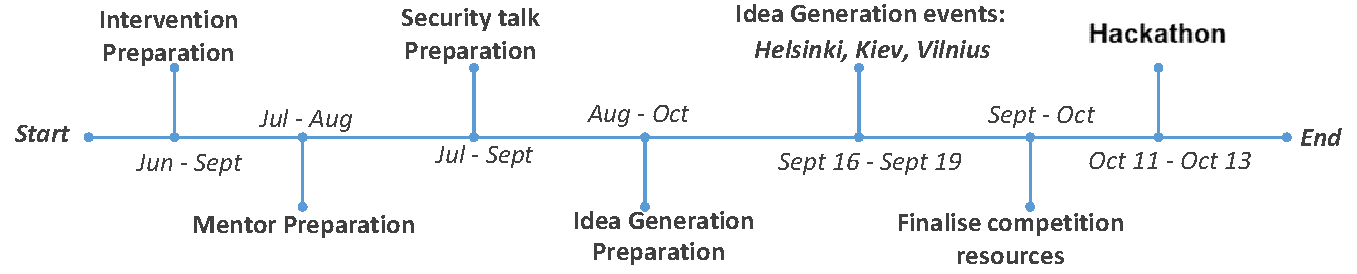
\includegraphics[width=\linewidth]{timelinehack.pdf}
  \caption{Timeline of the hackathon activities} \label{Fig:timeline} 
 \vspace{-10pt}
\end{figure}

\subsection{Data collection}
We selected three teams (denoted as A, B, and C) for our data collection. They were selected was based on their participation in the idea generation pre-hackathon events. The selected team characteristics are summarised in Table \ref{tab:teamcharacteristics}. For each team we collected observational data, questionnaires, and post-hackathon interviews. We will elaborate on how each data point contributes to answering our main research questions.

\begin{table}[h]
\vspace{-10pt}
    \caption{Team Characteristics}
    \label{tab:teamcharacteristics}
    \centering
    \begin{tabular}{|p{0.08\linewidth}|p{0.12\linewidth}|p{0.24\linewidth}|p{0.53\linewidth}|} \hline
	 Team & {\#} team members & Interview participants & Selection criteria \\ \hline
      A  & 6 & A01 (team lead), A02 (lead developer) &  No participation in idea generation pre-hackathon event. \\ \hline
      B  & 6 & B01 (team lead), B02 (security expert and developer) &  Participation in idea generation pre-hackathon event and continued with the same idea at hackathon. \\ \hline
      C  & 5 & C01 (team lead), C02 (developer) & Participation in idea generation pre-hackathon event but did not continue with same idea at hackathon. \\ \hline
    \end{tabular}
     \vspace{-10pt}
\end{table}

At the hackathon event, we moved between the teams to observe the participants. The observation method included monitoring at intervals and recording the responses of the participants to the interventions to influence learning in security.
Reactions such as attentiveness to security talks, positive interactions between teams and mentors reported when discussing with a sample of participants, and perceived satisfaction of participants related to their project indicated reactions to respective interventions. We also recorded other aspects that may contribute to understanding the learning experience of the participants, such as teamwork, team process, and leadership influence. 
We did not observe all teams throughout the entire duration of the hackathon as we perceived the early, mid and late phases of the hackathon to be most crucial.
We use the recorded observations to evaluate if the participants able to achieve learning gains with the introduced interventions as well as other team aspects (\hr{RQ1}). 

After the hackathon event, we conducted a post-hackathon questionnaire using pre-existing instruments validated and used to study hackathons\cite{van2015scrutinizing,filippova2017diversity,bhattacherjee2001understanding}, and adapted to our hackathon study\footnote{Detailed questionnaire information can be found in \url{https://github.com/alexandernolte/Collabtech2020_HackathonCybersecurityLearning/blob/master/questionnaire-scales.docx}}. The questionnaire covered the participants' perception of learning gains from the interventions, learning benefits from completing the security project. We also recorded participants' perception of specific team properties such as size, team familiarity, leadership, skill diversity, product satisfaction and collaboration process. These properties have been seen from prior work\cite{filippova2017diversity} to encourage learning at a hackathon. 
%Sample questions include; 
%\begin{enumerate}
%    \item To what extent was your decision to participate in the security hackathon motivated by:[\textit{options list}]
 %   \item How did you work together on your project during the hackathon? [\textit{options list}]
 %   \item To what extend do you agree with the following statements about your security learning experience at the hackathon? [[\textit{options list}]: \textit{Talking with my mentors helped me learn more about security}]
%    \item Please indicate your level of agreement with the following statements related to the satisfaction with your learning experience: [\textit{options list}]
%\end{enumerate}

From the selected teams, we chose 2 participants per team for an interview to discuss the hackathon experience, learning gains at the hackathon, and the hackathon outcome (i.e., security project worked on). 
These participants were selected because they either held a vital role in the team (i.e., team lead) or by observation, appeared to contribute significantly to the team.
%and analyzed for participants to provide a better comprehension of perceived individual and team learning experiences. (\hr{RQ2})
The interviews lasted between 25 and 30 minutes.
A sample of questions asked during the interviews include;
\begin{enumerate}
    \item How was the hackathon from your perspective in the form of: What did you do after you arrived? How did you see the event play out? 
    \item Did you attend the idea generation pre-hackathon event? What idea did you develop? How else did you prepare for this hackathon?
    \item What were the outcomes as a result of learning? [mentors, security talks, team members, working on the project]
    \item How do you perceive the outcome of the hackathon? Were you satisfied? How did you see your teamwork? 
    %\item What security issues did your project address? What security considerations did you place on the [process of creation of the product, the outcome of the project].
    \item Did you discover new security knowledge during the hackathon? How did you discover this?
    \item What about the continuity of your project? Have you use anything learned during the hackathon already? Are you planning to use it in the future? 
    %\item Do you still use any security knowledge gained during the hackathon?
\end{enumerate}
The data from the post-hackathon interviews allowed us to evaluate how the different interventions related to security learning thus enabling us to develop suggestion on how to improve the proposed interventions (\hr{RQ2}).

\subsection{Analysis procedure}\label{Sec:analysisprocedure}
First, we discuss the journeys of each selected team and the impacts of the introduced interventions on each teams based on a combination of observation, questionnaire, and interview results. The questionnaires are used qualitatively as an additional data source to the analysis procedure. %The overall analysis provides us with background information on the teams' activities during the hackathon.

We then compared security learning for the teams using Bloom's taxonomy learning dimensions as a basis \cite{bloom1956taxonomy,krathwohl2009taxonomy}.
Bloom's taxonomy describes levels of learning where each category of \textit{remember}, \textit{understand}, \textit{apply}, \textit{analyze}, \textit{evaluate}, and \textit{create} form the learning dimensions \cite{bloom1956taxonomy,krathwohl2009taxonomy}.
Our application of Bloom's taxonomy is based on data from team observations. A security expert assessed the learning gains for each team. By comparing the teams journeys, we can analyse how the participants encountered and worked with knowledge provided through the interventions.

Lastly, we evaluated how well the interventions worked for the team participants in encouraging perceived security learning using data from the questionnaires and interviews. This also reveals the shortcomings of the introduced interventions in fostering learning, where we suggest improvements to the interventions.

\section{Findings}
This section outlines the journeys of each selected team, the perception of each learning intervention for each team, and the differences between teams in relation to their learning process. Data collected about the perception of learning from interventions are illustrated in figure \ref{Fig:interventionsurvey}, while table \ref{tab:teamprop} shows data about team properties (of size, team familiarity, leadership, skill diversity, collaboration process, and product satisfaction).

\begin{figure}[h]
%\vspace{-10pt}
  \centering
  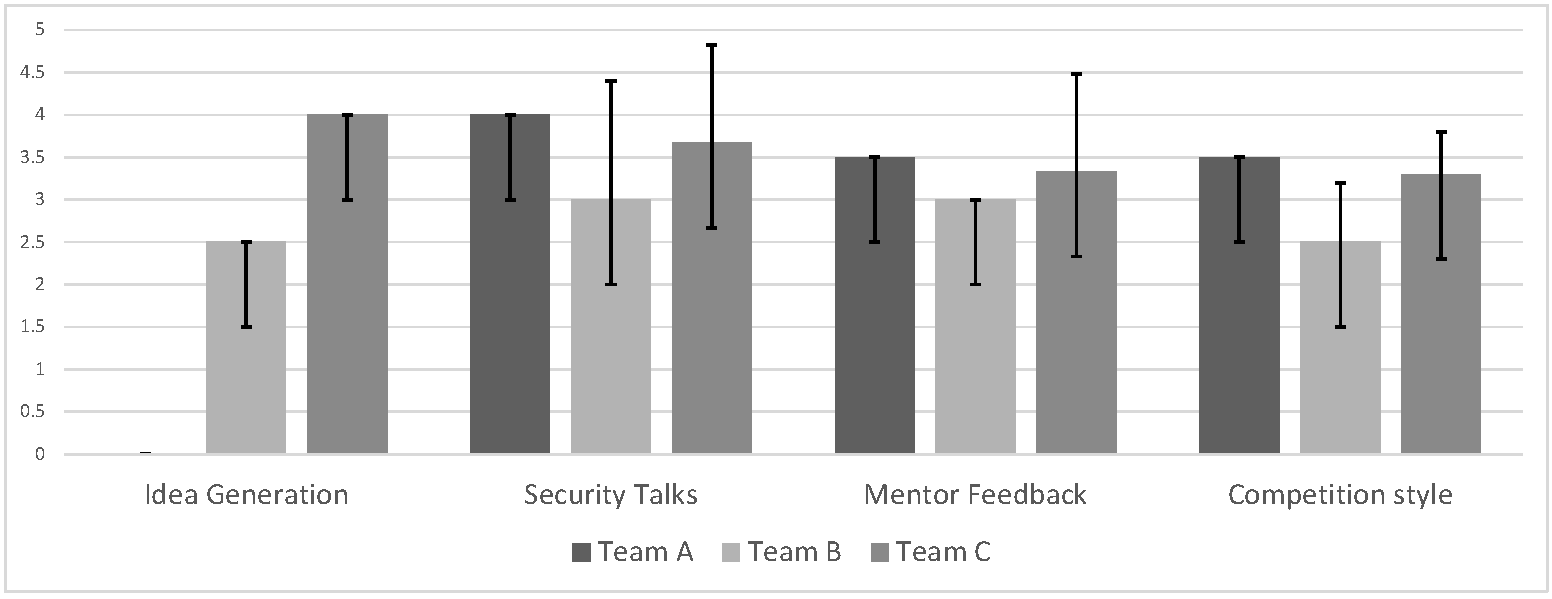
\includegraphics[width=1\linewidth]{interventionsurvey.pdf}
  \caption{Questionnaire responses by participants after the hackathon about interventions and satisfaction with learning experience. All responses were given on a 5-point scale which were anchored between strongly disagree (1) and strongly agree (5). The bars indicate the mean (m) and standard deviation (SD) for each team.} \label{Fig:interventionsurvey} 
% \vspace{-5pt}
\end{figure}

\begin{table}[h]
  %\vspace{-5pt}
    \caption{Calculated team property data (means, standard deviations, diversity formula, size count) used in qualitative analysis. Mean and standard deviation values are from responses given on a 5-point scale.}
    \label{tab:teamprop}
    %\centering
    \begin{tabular}{|p{0.25\linewidth}|p{0.24\linewidth}|p{0.24\linewidth}|p{0.24\linewidth}|}\hline
	Team property  &  Team A & Team B & Team C \\ \hline
	 size* & 6 & 6 & 5  \\\hline
	team familiarity & $m=1.1, SD=0.25$& $m=4, SD=0.9 $& $m=1, SD=0$  \\ \hline
	leadership& yes & yes & yes  \\ \hline
	skill diversity** & 0.6 & 0.7 & 0.4  \\ \hline
	collaboration process & $m=3.8, SD=0.3$ & $m=4.5, SD=0.4$ & $m=4, SD=0.3$ \\\hline
	product satisfaction & $m=4, SD=0.9$ & $m=2.9, SD=2.1$ & $m=3.5, SD=0.9 $ \\ \hline
    \end{tabular}
    *Reported number of participants in a team. \\
    ** To estimate skill diversity, we calculated similarities in the reported skills within a team and then determined how different they are (by subtracting the similarity value from one).
     \vspace{-10pt}
\end{table}

\subsection{Team A}
The leader of team A (A01) proposed the idea for the project in the idea generation session at the main hackathon event. A01 derived the idea from ``\textit{a security problem from studies}'' (A01) of the hackathon and intended to create a tool for enterprises to visualize security aspects. A01 formed a diverse (\textit{0.6}) 6-member team. The team members did not know each other before the hackathon ($m=1.1, SD=0.25$).
``\textit{Ideation continued during the hackathon because the idea was not properly prepared}'' (A01), and completed after discussions in the team and mentor feedback. The idea was refined to ``\textit{be targeted at company risk management team to help visualise and communicate security risk scenarios to upper management}'' (A01).

At the security talk sessions, team A members reported learning gains from the talks ($m = 4,SD=0$) and showed an understanding of the security domain while moving forward with the project. A01 highlighted on the ``\textit{educating experience about risk management and what is missing in the cybersecurity field}'' (A01) presented at the security talks.

During the creation of the final product, A01 highlighted that there was ``\textit{support by experienced team members to complete tasks}'' for the project. The team leader (A01) fostered learning within the team ``\textit{holding everything together, monitoring and identifying the needs of each team members for completing tasks}'' (A01). A01 described how teamwork grew and how ``\textit{everybody was eager to work and contribute in any way they could}''; ``\textit{some team members had no prior experience to security, but they tried to learn and contribute}'' (A01). A01 also reported that the team members ``\textit{went definitely beyond their current skills}'' (A01). The team leader (A01) was involved in  ``\textit{monitoring and identifying the needs of each team members for completing tasks}'', and mentors supported these responsibilities were necessary to adjust scoping of the project. A01 presented updates to the mentors about the project progress, getting feedback from mentors about moving forward to the prototype stage. Talking and interacting with mentors was reported to help the team learn more about security ($m = 3.5,SD=0.7$).

At the end of the hackathon event, team A presented the security prototype to judges for evaluation. Although team A did not win a prize at the competition, the team members reported, a moderate learning experience from building the final product ($m = 3.3,SD=0.7$) as an impact of the competition style design. But, there was a moderate agreement on the satisfaction with the product outcome ($m=4, SD=0.9$). A01 expressed that there will be no continuation in the project because ``\textit{the market value for this type of project}'' (A01) was unclear.%, having less intent to continue with the project as opposed to another team member A02.

\subsection{Team B}
The leader of team B (B01) presented an idea developed at the pre-hackathon event. B01 highlights that attending the idea generation event provided ``\textit{a lot of support to [my] idea}''. The idea developed was to ``\textit{make data security more desirable for startups and give them a badge}'' (B01), thereby aiming to improve security learning in startups. B01 presented the idea during the idea pitching session of the hackathon event and received feedback by mentors. 
After idea generation, B01 reports that team formation was easy. This is because B01 ``\textit{was familiar with most of the team because [we] studied together at the university}'' (B01) ($m=4, SD=0.9$). B01 formed a diverse (\textit{0.7}) 6-member team.

At the security talk sessions, B02 explained that these talks were instrumental as the team ``\textit{tried to gather all sorts of information on how to secure systems and gained knowledge}'' (B02). Team B members reported security gains from the talks ($m = 3,SD=1.4$). Team B participants reported learning experiences from the mentor feedback ($m = 3,SD=0$) as it provided ``\textit{an opportunity for [us] to explain our work progress}'' (B02). 
B02 reported that ``\textit{different mentors visited multiple times}'', and that the mentors ``\textit{visited to guide completing tasks}'' (B02), but B01 reported that the multiple visits ``\textit{disrupted the flow of tasks}''(B01). B01 reported that mentors specifically provided feedback on the scoping of the project, and refinement of project content. % to define the life-cycle of different startups and the security implementations needed for each stage of the life-cycle as well as the business aspects.

During the creation of the final product, the team perceived their collaboration process to be efficient ($m=4.5, SD=0.4$). B01 mentioned that a ``\textit{blackboard equipment for documenting the team's process and ideas, allowing [us] to see the big picture}'' (B01), thereby aiding collaboration between members of the team and between the team and visiting mentors. 
On the impact of competition style of the hackathon on team B, there was a moderate learning experience($m = 2.5, SD=0.7$) from accomplishing the task of building security content for the prototype.

Towards the end of the hackathon event, Team B pitched their project and presented the prototype for evaluation. Team B won a prize for a unique product developed and its perceived usefulness to the security community. Interestingly, there was a moderate satisfaction with the outcome of the project ($m=2.9, SD=2.1$). 
B01 raised an issue with a team member leaving the team unexpectedly halfway through the hackathon with the resources already gathered by the team. Continuation of the project following the competition style intervention was encouraged by the incentive prize awarded to the team project. Although B01 reported that the team intends to continue with the project, we learned from both B01 and B02 that the provided incentive might not be useful to its continuation.


\subsection{Team C}
The team lead (C01) pitched an idea during the idea generation session of the hackathon event. Although C01 attended the idea generation pre-hackathon event, the idea pitched at the main hackathon event was different from the one C01 worked on during the pre-hackathon event. C01 pitched the idea to ``\textit{create a binary betting platform for smart contracts}''(C01) on a blockchain platform. However, mentors provided feedback that the presented idea did not readily provide a project addressing current security issues and asked C01 to think more about potential security aspects of that idea. C01 formed a less diverse ($\textit{0.4}$) 5-member team, consisting mainly of developers interested in developing a blockchain-based project.

Once team formation was complete, the participants in team C continued idea refinement with the mentor feedback. C02 stated that the initial idea ``\textit{didn't seem like a good idea for a security hackathon, so [we] needed to connect it to a security topic}'' (C02). Thus, a new idea was formed based on blockchain, where the team decided on ``\textit{an availability insurance smart contract for service providers}'' (C02). The team leader (C01) provided progress reports on development to the mentors, who contributed feedback on how to enhance the proposed security prototype. The participants of team C reported learning experience from the provided mentor feedback ($m = 3.33,SD=1.15$). Although there were no individual reports from the participants of team C about learning experiences from the security talk sessions, questionnaires responses from team C participants report learning gains from the security talk intervention ($m = 3.67,SD=1.15$).

The participants in team C report security learning experience by working on project tasks ($m = 3.3,SD=0.5$) such as researching the security aspects of the prototype. The team perceived their collaboration process to be efficient ($m=4, SD=0.3$). C02 highlighted that this was due to the team's high interest in development using blockchain. Towards the end of the event, Team C pitched the final prototype for evaluation. After evaluation, Team C did not win a prize at the event and reported satisfaction with the outcome of the project ($m=3.5, SD=0.9$). C02 mentioned that there were no intentions of the participants to continue with the project idea.

\subsection{Team comparison} \label{teamcomparison}
In this section, we compare the learning gains between the teams A, B and C based on the knowledge of the team's activity, and other observations at the hackathon (see section \ref{Sec:interventions}). Figure \ref{tab:bloomteamcomp} shows the learning gains based on Blooms taxonomy.
According to our findings, team B showed the most learning gains followed by team A then team C. In the following, we discuss how the teams were observed to use the different interventions in order to achieve learning gains.

Team A was showed the ability to recognise relevant security knowledge and to provide specific security information gained through the security talks. The study participants (A01, A02) were able to recall the security risk management concepts discussed in the security talks, and discussed about these concepts in relation to their security project. 
Team B also showed the ability to remember security knowledge from the security talks intervention. B01 presented the security idea of a platform that encourages data security, related to security issues raised in the security talks. Team C participants talked about the availability security aspects of blockchain, recalling knowledge from security talk sessions. Teams A, B, and C thus attained the \textbf{remember} process category.

Teams A and B showed the ability not only to remember and recall but interpret and explain security concepts. Team A showed an understanding of security issues from the security talks. This understanding is evident in the generation of a security-relevant idea and discussions with mentors on security issues and their impact in a security risk-aware business environment. Team B showed an understanding of security concepts, evident in the generation of a security-relevant project for the start-up environment. Thus the teams' A and B attained the \textbf{understand} process category.

Teams A and B were able to apply the security knowledge gained during the idea generation sessions, following mentor feedback and in the process of building a unique security project.
Team A (A01) was able to incorporate feedback from mentors to focus on resources to visualise and communicate security risk scenarios. Team B (B01) was able to apply mentor feedback in defining the security aspects within the life-cycle of target start-ups. Team B also showed the application of security knowledge gained by research on the security aspects within start-up life cycles. Team C participants, in interviews, did not readily show the application of gained security knowledge in its process and blockchain based product. Thus, teams A and B attained the \textbf{apply} process.

Teams A, B, and C were given the chance to present their developed security prototypes. However, only team B was able to show how the security knowledge gained through interventions related to the overall purpose and structure of their project. Team B respondents presented an analysis of how the introduction of each intervention affected each task, sub-task or process in the development of the final prototype. The team B achieved the \textbf{Analyse} process. 
\begin{comment}
\begin{table}[h]
\vspace{-5pt}
    \caption{Team Learning Comparison}
    \label{tab:bloomteamcomp}
    \centering
    \begin{tabular}{|p{0.15\linewidth}|p{0.14\linewidth}|p{0.14\linewidth}|p{0.12\linewidth}|p{0.12\linewidth}|p{0.13\linewidth}|p{0.14\linewidth}|}
    \hline
	 & Remember knowledge & Understand knowledge & Apply knowledge & Analyse knowledge & Evaluate knowledge & Create knowledge\\ \hline
	Team \newline Knowledge & A, B, C & A, B & A, B & B & -- & -- \\ \hline
    \end{tabular}
   % \vspace{-15pt}
\end{table}

\end{comment}

\begin{figure}[h]
%\vspace{-10pt}
  \centering
  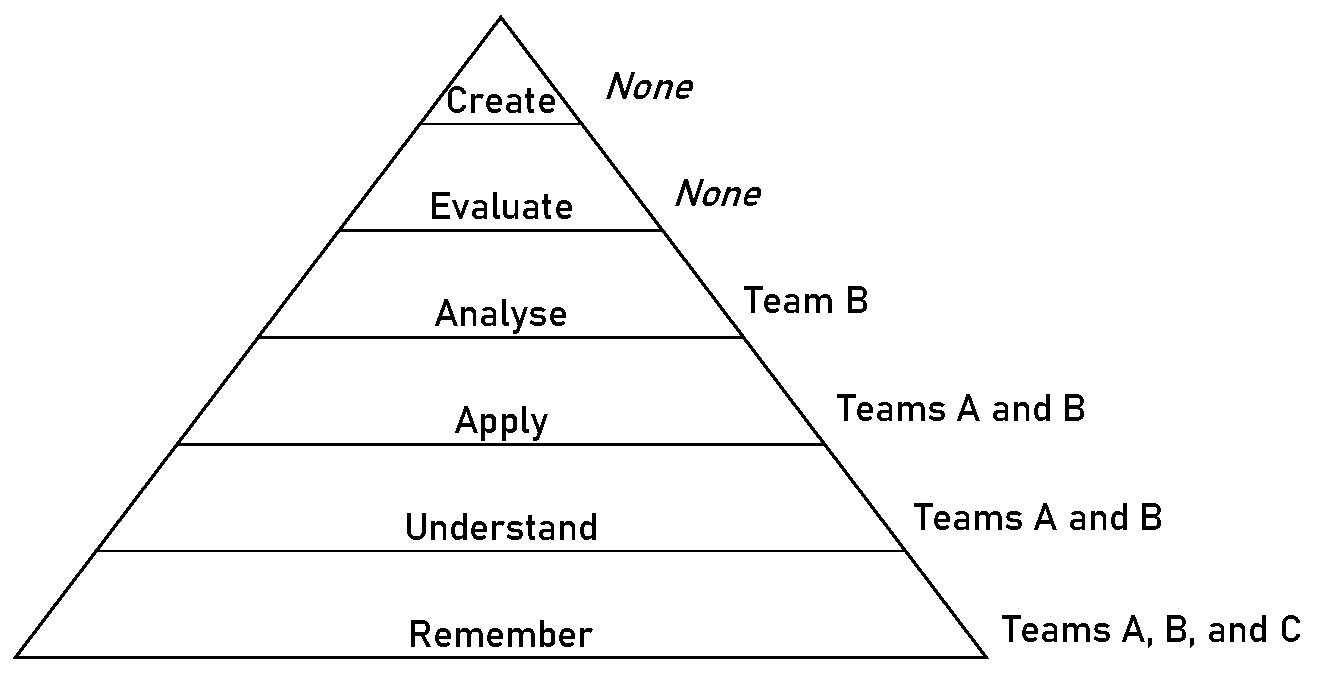
\includegraphics[width=1\linewidth]{Bloomsoutput.pdf}
  \caption{Team Learning Comparison} \label{tab:bloomteamcomp} 
% \vspace{-5pt}
\end{figure}

\section{Discussion}
In this section, we evaluate how the teams A, B, and C benefited from the different proposed interventions. Relating those with the previously discussed differences related to the teams' learning gains allows us to develop improvements for the interventions thus answering \hr{RQ2}.

\subsection{Evaluation of interventions} \label{evalintervention}
Our findings indicate that Team B benefited the most from the \textbf{idea generation} intervention as it was instrumental in creating the security project, and as a result, winning the competition. Of all three teams, team B was able to take the most advantage of this intervention, and having more time to work on their idea, resulted in a more mature security idea they could work on during the main hackathon. Team B reported that this was possible because the team lead (B01) attended the idea generation sessions at the pre-hackathon event and began developing their project idea already then.
Although C01 attended the idea generation sessions at the pre-hackathon event, C01 ended up working on a new idea during the main hackathon. Also, none of the participants of team A attended the pre-hackathon event.
As such, these teams had fewer chances in involving in as much security learning from idea generation as team B.


Teams A and B benefited most from \textbf{security talks} while team C showed little to no benefit according to our findings. This could be because the security talks provided were mainly related to teams A and B's security projects. 
A01 reported that the security talk on security risk management was relevant to their security risk visualisation project. B01 reported that the security talk on start-up security learning provided the required security knowledge relevant to the team's project.
C01 reported that the security talks were not particularly relevant to their blockchain project but were only useful to provide general security knowledge. It thus appears important that talks need to be tailored towards team needs in order to be perceived as useful.

Our findings also indicate that Team B benefited most from the \textbf{mentor feedback} intervention in achieving security learning as opposed to other teams. This could be because of the high amount of interaction with diverse mentors. B02 reported that different mentors visited the team at multiple times to provide an expert perspective on work progress. However, B01 said that mentoring became disruptive to the team process because of multiple visits.
Teams A and C, showed little benefit from this intervention and did not report as much interaction with diverse mentors as with team B. 
A01 reported mentor interaction in idea generation and in supporting the completion of set tasks for the security project, while C01 only reported mentor interaction related to idea generation. Thus, reducing the teams' chances of involving in as much security learning as team B. 
It appears crucial that we should organise mentoring appropriately to ensure an adequate amount of mentor interaction.

Related to the \textbf{competition style} intervention, Team B benefited the most. B01 reported that the intervention encouraged rapid knowledge gathering and application of the security knowledge to product creation, thus winning a prize at the hackathon.
The perceived benefit could also be as a result of culminating factors including idea generation, team formation, and team properties such as team familiarity, collaboration, satisfaction and leadership, all within the competition constraints. Teams A and C showed little benefit from this intervention.
A01 reported that they did not win a prize because too much time was spent on idea generation, causing a race with time to complete the security project adequately. C02 also reported difficulties faced in idea generation.

\subsection{Suggestions for improvement}
Based on our analysis we developed the following suggestion to improve the four main interventions introduced in section \ref{Sec:interventions} thus answering \hr{RQ2}.

Based on our findings we would suggest to support teams to develop ideas prior to the main event and continue coaching them related to this idea throughout. Changing an idea does not appear to be feasible.
%\subsubsection{Security talks.}
For \textbf{security talks}, three suggestions can be proposed for future iterations based on our findings.
First, the content of the security talks can be more domain-generic. Another option is to appropriately scope the ideas generated at the hackathon to the context of the hackathon. Finally, we develop the security talks only after idea generation is completed, so that the talks are more domain-specific and have maximum effect of offering adequate security knowledge to participants.
%\subsubsection{Mentor feedback.}
Based on our findings, we suggest that the \textbf{mentor feedback} intervention be handled with excellent coordination not to disrupt the team process. 
We suggest that a designated member of the team (most likely the team leader) with knowledge of the team's process, stand in between the mentors and the team when necessary, to handle explanations of the teams progress, and what the team needs in mentoring to prevent multiple disruptions.
%\subsubsection{Competition style.}
%In the \textbf{competition style} we suggest 
%However, B01 reported that the incentive provided was not relevant to the needs of the specific product because the product was content-specific, and thus, building the content and adapting it to the needs of real-life stakeholders was a priority over marketing. B01 stated that they ``\textit{expected to have interviews and discussions with stakeholders and startups to build proper security content, but the program did not provide this}". A suggestion is to understand the future needs of a project and provide an incentive that accommodates these needs.

\subsection{Limitations}
The aim of our study was to develop and evaluate specific interventions that can foster security learning during a hackathon. While it appeared reasonable to conduct an action research study \cite{lewin1946action} there are certain limitations associated with this particular study design. We developed specific interventions and studied three teams that participated in a hackathon over a limited period of time that had specific backgrounds and goals for attending the hackathon. Despite selecting teams thoroughly it is not possible to generalize findings beyond our study context since studying a different setting with different teams, during a different hackathon working on different projects might yield different results. Moreover the researchers conducting the study were involved in the planning of the hackathon which can affect the reported findings despite our best efforts to refrain from interfering during the hackathon itself. We also abstained from making causal claims instead providing a rich description of the observed behavior and reported perceptions of teams based on which we discuss differences in how they reacted to the different proposed interventions.

\section{Concluding remarks}
In this paper, we reported on findings from an action research study of three teams at a security hackathon. The study aimed to propose and evaluate interventions specific interventions -- namely idea generation, security talks, mentor feedback and a competition-style event -- to foster security learning. Our findings indicate that the introduced interventions were beneficial to stimulate learning at different levels. For future hackathons, we propose to support idea generation of teams before a hackathon, thematic talks during a hackathon that are related to team projects, and organisation of mentors to increase interaction but prevent disruption. Our research also provides useful information to organisers who seek to encourage security learning in their hackathon events. 


\bibliographystyle{splncs04}
\bibliography{references}

\end{document}
